\documentclass{article}
\usepackage[utf8]{inputenc}
\usepackage[margin=1in]{geometry}
\usepackage{amsmath}
\usepackage{amssymb} %need this for boldface C
\usepackage{verbatim} %for inline code
\usepackage{indentfirst}

%For images
\usepackage{graphicx}
\usepackage{subcaption}
\usepackage[export]{adjustbox}
\usepackage{wrapfig}

\usepackage{float}

\setlength{\parindent}{4em}
\setlength{\parskip}{0.5em}

\title{CTA200 Assignment 2}
\author{Matthew Leung}
\date{May 8, 2020}

\begin{document}

\maketitle

\section{Introduction}

In this investigation, we will look at the Mandelbrot set and a system of ordinary differential equations (ODEs) used for infectious disease modelling in epidemiology.

\section{Mandelbrot set}
\subsection{Background}
Consider the set of points $S=\{c=x+iy \in \mathbb{C} \mid x \in (-2,2), y \in (-2,2), x,y \in \mathbb{R} \}$. For each point $c \in S$, let us iterate over the recurrence relation $z_{i+1} = z_i^2+c$, with $z_0 = 0$. If $|z| > 2$, then the sequence diverges. The set of points such that $z$ does not diverge is called the Mandelbrot set.

\subsection{Methods}
The Mandelbrot set was plotted on a 2-dimensional plot, with colours representing the iteration number $i$ at at which the sequence $z$ diverged for every point $c$. Using Python, and the Numpy and Matplotlib libraries, the Mandelbrot set was plotted. The set $S$ was represented using two $1 \times n$ Numpy arrays, for the values of $x$ and $y$, with $n=1000$. The Numpy  \verb|meshgrid()| function was applied to these two arrays to create a 2-dimensional mesh of the coordinates. This was then passed into a function to generate the iteration number $i$ for divergence for each $c$. Using a \verb|for| loop, the recurrence relation was repeatedly applied to every point using Numpy matrix operations on a $n \times n$ array representing $S$. Another $n \times n$ Numpy array was initialized, which stored boolean values of whether or not a certain point diverged. If it did, then the corresponding $i$ for each point that diverged would be stored in another $n \times n$ Numpy array, which the function would return. Note that the maximum number of iterations for the recurrence relation was selected to be 100. The results were then plotted using the Matplotlib library.

\subsection{Results}

The following figures show the Mandelbrot set, plotted using Python by the above method. Figure 1a shows the Mandelbrot set for $x \in (-2,2)$ and $y \in (-2,2)$, while Figure 1b shows the Mandelbrot set for $x \in (-2,0)$ and $y \in (-1,1)$. The colours show the number of iterations for divergence. From these colour plots, we can see that there is a fractal pattern. The points with darker colours are those that do not diverge. Figure 1c and Figure 1d show a binary black and white image of the Mandelbrot set. The points in black diverge, whereas the points in white are a part of the the Mandelbrot set. With a higher $n$, the fractal patterns will be more evident, with more detail.

\begin{figure}[H]
\centering
\begin{subfigure}{.5\textwidth}
  \centering
  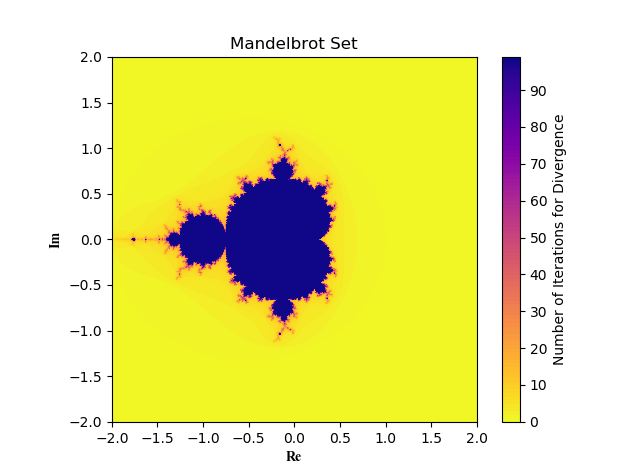
\includegraphics[width=\textwidth]{Mandelbrot_1.png}
  \caption{Colour map, $x \in (-2,2)$ and $y \in (-2,2)$}
  \label{fig:sub1}
\end{subfigure}%
\begin{subfigure}{.5\textwidth}
  \centering
  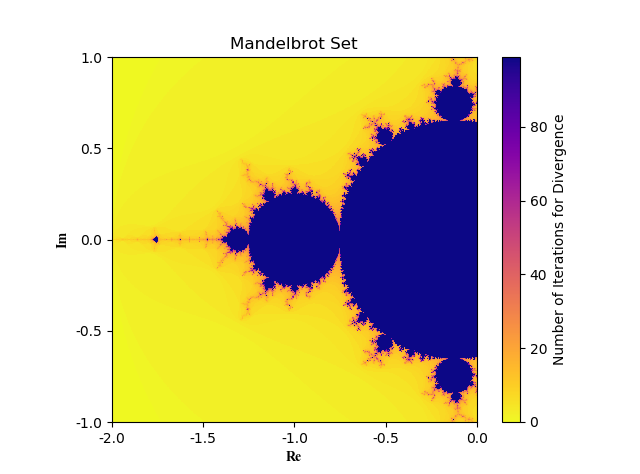
\includegraphics[width=\textwidth]{Mandelbrot_2.png}
  \caption{Colour map, $x \in (-2,0)$ and $y \in (-1,1)$}
  \label{fig:sub2}
\end{subfigure}
\begin{subfigure}{.5\textwidth}
  \centering
  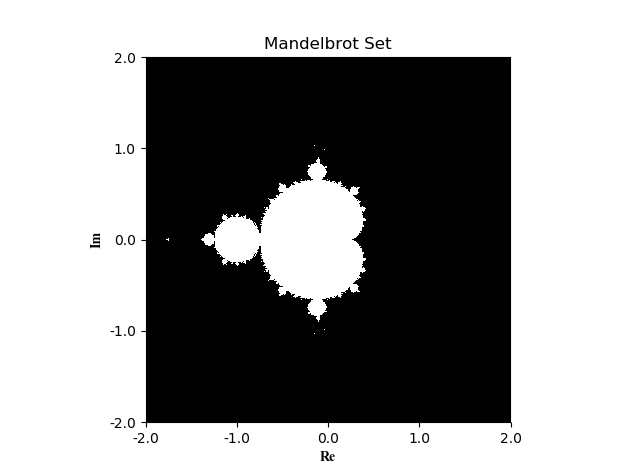
\includegraphics[width=\textwidth]{Mandelbrot_3.png}
  \caption{Black and white, $x \in (-2,2)$ and $y \in (-2,2)$}
  \label{fig:sub3}
\end{subfigure}%
\begin{subfigure}{.5\textwidth}
  \centering
  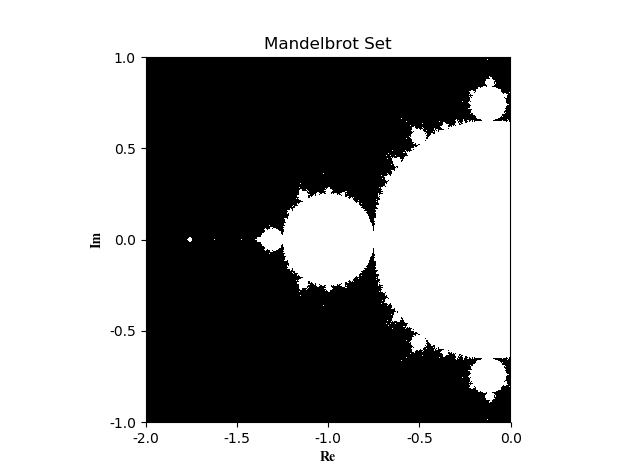
\includegraphics[width=\textwidth]{Mandelbrot_4.png}
  \caption{Black and white, $x \in (-2,0)$ and $y \in (-1,1)$}
  \label{fig:sub4}
\end{subfigure}

\caption{Mandelbrot set plotted in Python}
\label{fig:test1}
\end{figure}

\section{Epidemiology Models}
\subsection{Background}
The epidemiology model we will investigate is called the SIR model. In its most basic form, it consists of three system of ODEs, shown below. This models an infectious disease over time.
\begin{align}
    \frac{dS}{dt} &= -\frac{\beta S I}{N}\\
    \frac{dI}{dt} &= \frac{\beta S I}{N} - \gamma I\\
    \frac{dR}{dt} &= \gamma I
\end{align}
$S(t)$ is the number of people susceptible to the disease, who have not yet been infected. $I(t)$ is the number of infected people. $R(t)$ is the number of people who have recovered or who are deceased. $N$ is the total population size, $\beta$ is the average number of contacts per person per time, and $\gamma$ is the transition rate for people who are infected to become either recovered or deceased.

\subsection{Methods}
To solve this system of ODEs, and to plot each of the functions $S(t)$, $I(t)$, and $R(t)$, Python was used, along with the SciPy and Matplotlib libraries. SciPy's \verb|integrate.odeint()| function was used to solve this system of ODEs, with various values of $\beta$ and $\gamma$. The initial conditions were $I(0) = 1$, $S(0)=999$, and $R(0) = 0$. $N$ was set to be 1000 people, and the time $t$ was in the interval $t \in [0,200]$. The solutions to the ODEs were plotted using Matplotlib.

\subsection{Results}

\begin{figure}[H]
\centering
\begin{subfigure}{.5\textwidth}
  \centering
  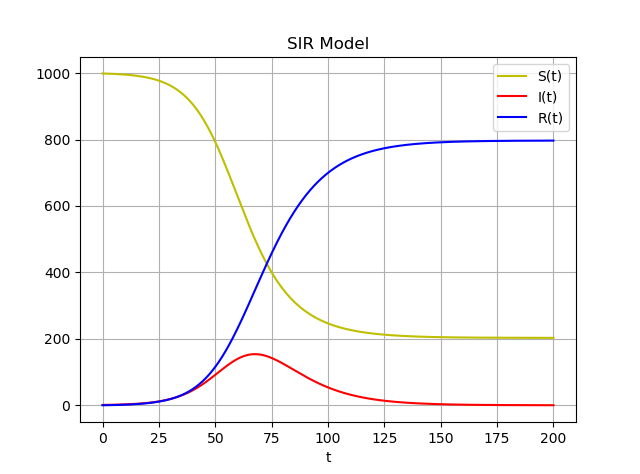
\includegraphics[width=\textwidth]{SIR_1.png}
  \caption{$\beta = 0.2, \gamma = 0.1$}
  \label{fig:sub5}
\end{subfigure}%
\begin{subfigure}{.5\textwidth}
  \centering
  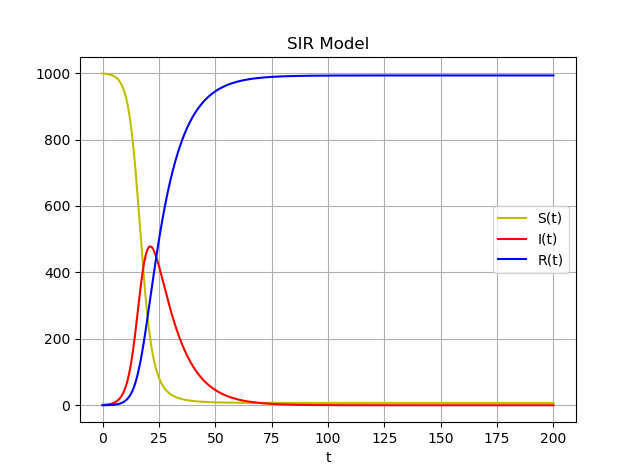
\includegraphics[width=\textwidth]{SIR_2.png}
  \caption{$\beta = 0.5, \gamma = 0.1$}
  \label{fig:sub6}
\end{subfigure}
\begin{subfigure}{.5\textwidth}
  \centering
  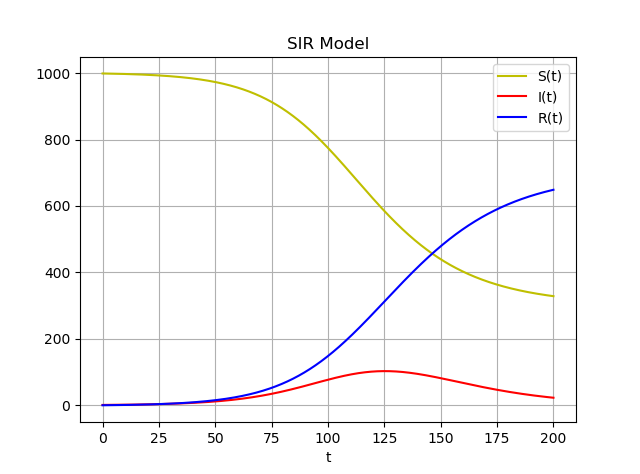
\includegraphics[width=\textwidth]{SIR_3.png}
  \caption{$\beta = 0.12, \gamma = 0.07$}
  \label{fig:sub7}
\end{subfigure}%
\begin{subfigure}{.5\textwidth}
  \centering
  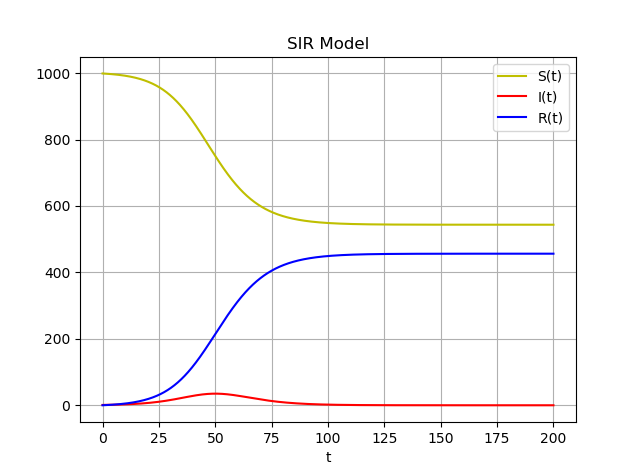
\includegraphics[width=\textwidth]{SIR_4.png}
  \caption{$\beta = 0.4, \gamma = 0.3$}
  \label{fig:sub8}
\end{subfigure}

\caption{SIR model with various $\beta$ and $\gamma$}
\label{fig:test2}
\end{figure}

Figure 2 above shows the solution of the system of ODEs for various $\beta$ and $\gamma$. Consider Figure 2b in comparison with Figure 2a. In Figure 2b, $\beta$ is larger, meaning that people have contact with others more frequently. This results in a larger amount of people being infected. If people have less contact with each other, then less people will become infected, as shown in Figure 2c. If $\gamma$ is higher, then that means that people will recover faster, and there will be less infections overall, as shown in Figure 4d. Figure 4c and Figure 4d show the concept of ``flattening the curve''. Decreasing $\beta$ and increasing $\gamma$ would cause less infections, with infections being spread out over a longer period of time.

This is especially relevant at the time of this report, during the current global COVID-19 pandemic. The SIR model here shows that social distancing (decreasing $\beta$) is effective in lowering the amount of people who are infected. In addition, if a vaccine is developed quickly, or if more people recover (increasing $\gamma$), then there will be less infections. However, the SIR model is very simple, and does not account for many other factors. The SIR model can be greatly elaborated.

\subsection{SIRD Model}
A slightly more elaborate version of the SIR model is the SIRD model. It is similar to the SIR model but with a few differences. We introduce a new function $D(t)$, which is the number of deaths in the population. $R(t)$ is strictly now the number of people who have recovered. $\gamma$ is now the recovery rate, and we introduce a new constant, $\mu$, which is the mortality rate. The SIRD model has the following system of ODEs.
\begin{align}
    \frac{dS}{dt} &= -\frac{\beta S I}{N}\\
    \frac{dI}{dt} &= \frac{\beta S I}{N} - \gamma I - \mu I\\
    \frac{dR}{dt} &= \gamma I\\
    \frac{dD}{dt} &= \mu I
\end{align}
Note that equations (4) and (6) are the same as equations (1) and (3) respectively. Equation (5) is the same as equation (2), but with an additional $-\mu I$ term. The number of infected people will also decrease if more people become deceased. Equation (7) is a new equation. Figure 3 below shows the solution for a SIRD model with the same initial conditions as the plots in Figure 2, but with $\beta=0.2$, $\gamma = 0.1$, and $\mu=0.02$. Note that $D(0)=0$.

\begin{figure}[H]
\centering
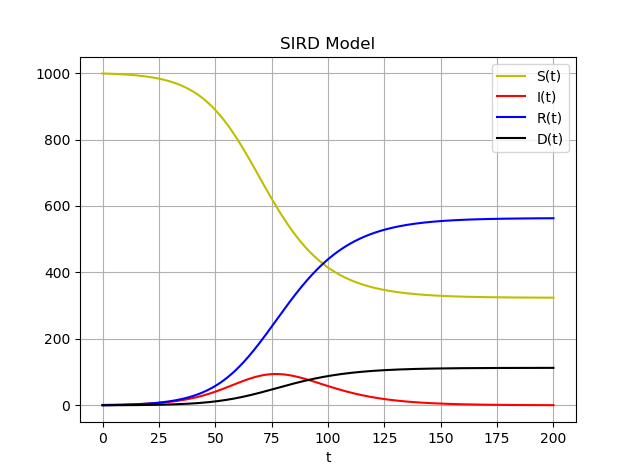
\includegraphics[width=0.5\textwidth]{SIRD_1.png}
\caption{SIRD model with $\beta=0.2, \gamma = 0.1, \mu=0.02$}
\label{fig:figure3}
\end{figure}

This model could tell us more information since the deaths in the population are separately accounted for. However, in reality, infectious diseases are much more complex, with many more factors, some of which cannot be truly accounted for. The SIR and SIRD models are just a basic picture of what could happen. A model is only as good as its assumptions.

\end{document}
